La première des alertes que nous proposons de traiter est l'alerte
dite du \emph{Grand Veymont,} issue de l'enregistrement d'un appel au
secours effectué par un accompagnateur en montagne, au sujet d'un de
ses clients.
%
Cette alerte est la plus simple est la plus courte de celles que nous
traiterons ici.

\subsection{Présentation de l'alerte}
\label{subsec:9-2-1}

L'alerte du \emph{Grand Veymont} est l'extrait, d'une durée de 1
minute 06, d'un appel effectué par un accompagnateur en montagne au
sujet d'un de ses clients \autoref{anx:retrans-gv-verb}.


Cette alerte est la plus courte de celles que nous présenterons ici,
elle est composée de 12 extraits, pour un total de 16 expressions.



Pas d'objets multiples

les indications données par le requérant sont assez précises et
détaillées, il est donc possible de définir une \emph{zone initiale de
  recherche} de petite taille. Nous avons défini une \ac{zir} de
\SI{25}{\kilo\meter\squared} (\autoref{fig:zir_grand_veyont}).

\begin{figure}
  \centering
  \begin{tikzpicture}
  \tikzset{et/.style={above,font=\footnotesize\vphantom{Ag}}}
  %
  \node[inner sep=0pt, anchor=south west] (image) at (0,0){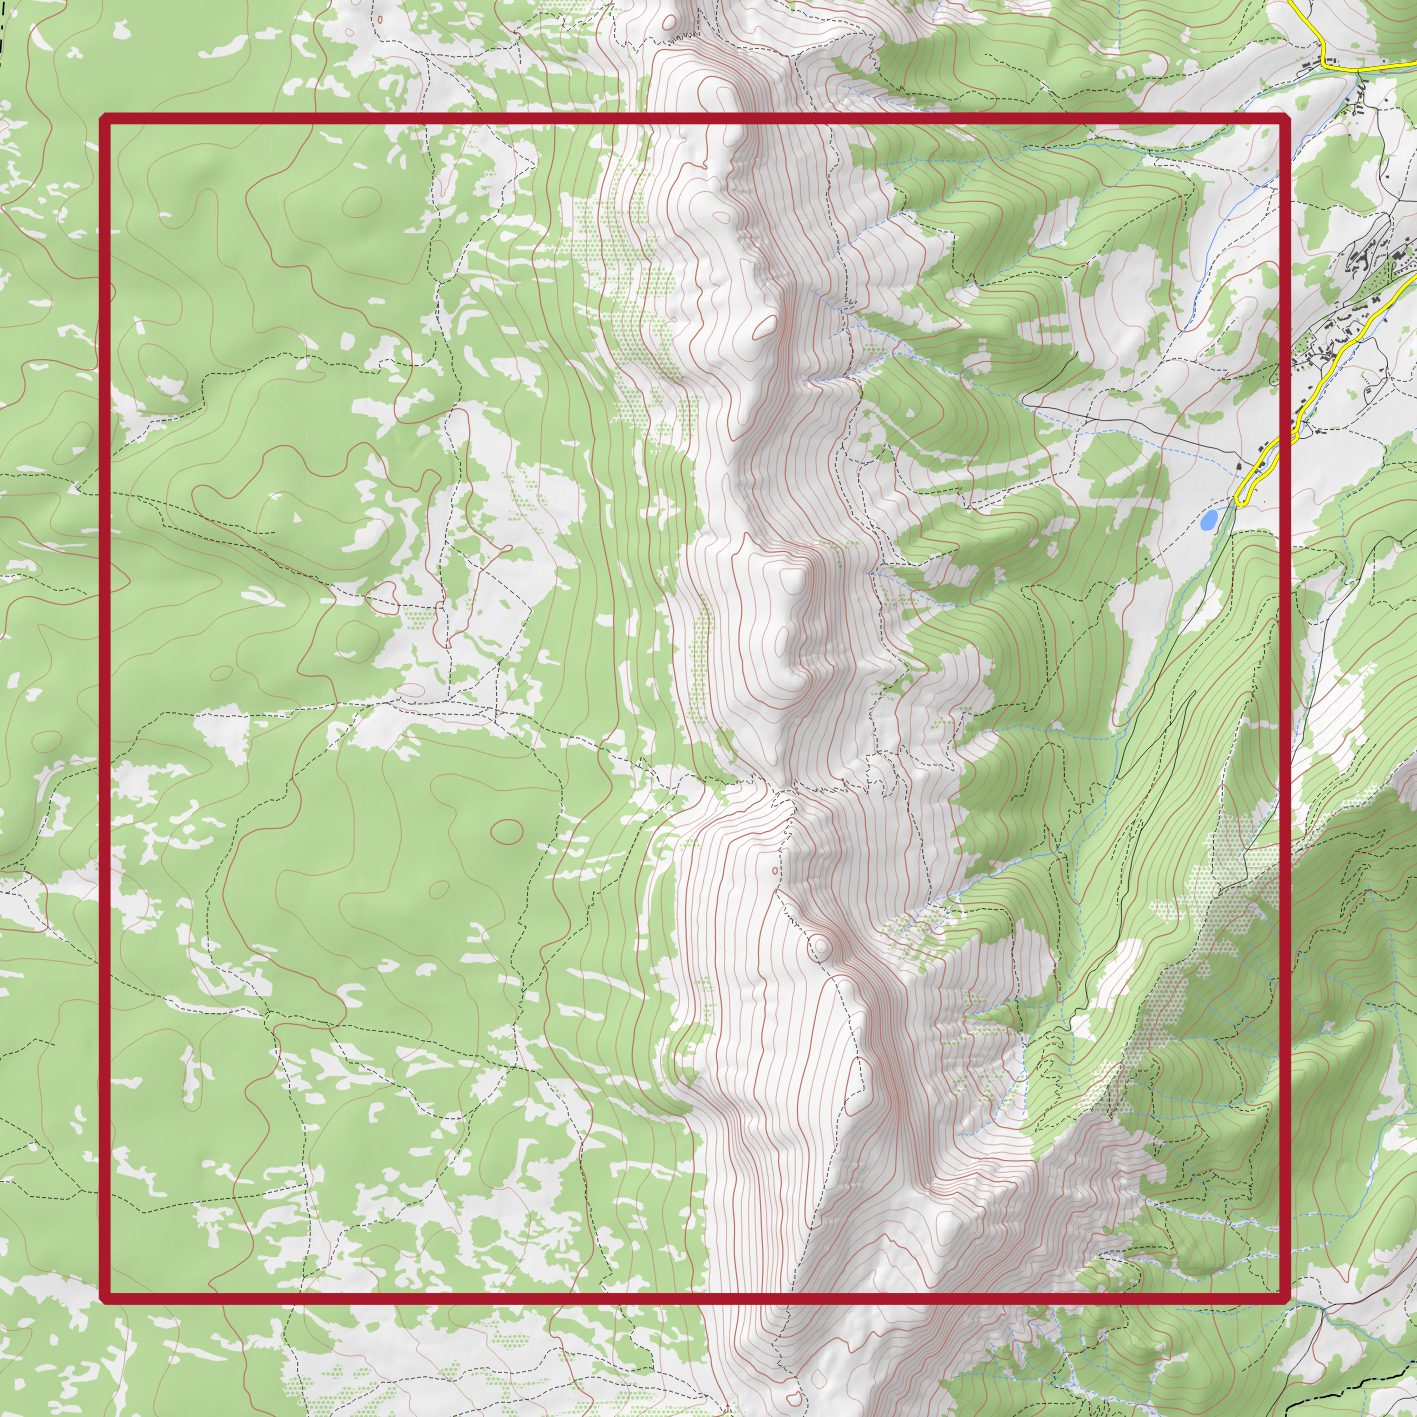
\includegraphics{./figures/ZIR_grand_veymont.png}};
  %
  \begin{scope}
    \node (P2) at ([yshift=-.5cm]image.south east) {};
    \node (P1) at ([yshift=-.5cm]image.south west) {};
    %
    \foreach \x [evaluate=\xshift using \x/10, evaluate=\rad using (\x * .0004) + .01] in {0,...,100}
    {
      \draw[fill=black,draw=none, below] ([xshift=\xshift cm, yshift=-.5cm]P1) circle [radius=\rad cm];
    }
    %
    \path(P1 |- 0cm,-1cm) --++ (10,0)
    node[et,pos=0] {0}
    node[et,pos=.1] {0,1}
    node[et,pos=.2] {0,2}
    node[et,pos=.3] {0,3}
    node[et,pos=.4] {0,4}
    node[et,pos=.65] {0,65}
    node[et,pos=1] {1};
    % Échelle
    \draw[-] (P2 |- -1cm,-1cm) --++ (-1,0) node[et,pos=.5] {\SI{500}{\meter}};
    % Légende détaillée
    \path (P1) -- (P2) node[pos=.5, yshift=-1cm] {\tiny Pour la légende détaillée du fond topographique voir \autoref{anx:topo_leg}. Sources: BD TOPO 2018, BD ALTI 2018.}; 
  \end{scope}
\end{tikzpicture}
  \caption{Zone initiale de recherche pour l'alerte \enquote{Grand Veymont}}
  \label{fig:zir_grand_veyont}
\end{figure}


\subsubsection{Retranscription et identification des indices de localisation}
\label{subsec:9-2-1-1}


Le verbatim de l'enregistrement audio de l'alerte \emph{Grand Veymont}
est donné dans la \autoref{anx:retrans-gv-verb}.
%
Comme nous l’expliquions dans le \autoref{chap:05}, 


L'alerte commence par deux extraits (\nex{1} et \nex{2}) décrivant
le contexte de la descente :
%
\begin{dialogue}
  % 
  \Req \nex{1-1} J'ai eu du mal à descendre entre le sommet du grand
veymont et là où je suis. \nex{2-1} La descente était très très lente.
\end{dialogue}
%
Ces deux informations sont de la configuration, elles ne correspondent
donc pas à un indice de localisation




Viennent ensuite les extraits \nex{3} et \nex{4} qui donnent beaucoup
d'informations :
%
\begin{dialogue}
  %
  \Sec \nex{3-1} Vous êtes entre \emph{Grand Veymont} et \emph{Pas de
la Ville} ?

  \Req \nex{3-1} Je suis entre le \emph{Grand Veymont}
\textins{\nex{4-2} sous le \emph{Grand Veymont}} et \emph{Pas de la
Ville,} tout à fait, \nex{4-3} coté sud.
\end{dialogue}
%

La description donnée par le requérant (\nex{4-3}) étant
incohérente, le secouriste en demande la confirmation (\nex{5-1}) :
%
\begin{dialogue}
  %
  \Sec \nex{5-1} Côté Sud du \emph{Pas de la Ville} ?
%
  \Req \nex{6-1} Non, côté Nord.
\end{dialogue}
%
Ces deux extraits contredisent clairement l'expression \nex{4-3}

On peut déduire de ces extraits (\nex{4-3, 5-1, 6-1}) que le requérant
est situé au
%
On peut donc envisager d'utiliser la relation de localisation
\onto[orl]{Au\-Nord\-De} pour spatialiser cet indice de
localisation. Cependant, cette relation correspond au regroupement de
deux autres relations \onto[orl]{Dans\-La\-Partie\-Nord\-De} et
\onto[orl]{Au\-Nord\-De\-Externe}, dont l'usage peut être ici plus
pertinent.
%
La relation de localisation \onto[orl]{Dans\-La\-Partie\Nord\-De}
décrit une situation où la cible est située à \emph{l'intérieur} du
site et dans sa partie nord.
%
Rien dans la situation décrite par le requérant n'indique qu'il serait
situé dans le site
%
La relation de localisation \onto[orl]{Au\-Nord\-De\-Externe} décrit
quant à elle une situation où la cible est au nord du site, sans être
ni contact, ni au sein de celui-ci.
%
Dans le contexte



\begin{dialogue}
  % 
  \Sec \nex{7-1} Vous êtes au-delà du \emph{Pas de la Ville} ?
  \nex{7-2} Entre \emph{Pas de la ville} et \emph{Pierre Blanche ?}
  % 
  \Req \nex{8-1} Oui, je suis au-delà du \emph{Pas de la Ville.}
\end{dialogue}



\begin{dialogue}
  %
  \Req \nex{9-1} Sur une zone à peu près plate et
  caillouteuse. \nex{10-1} Sur une petite prairie.
\end{dialogue}


La dernière partie de l'alerte est composée des extraits \nex{11-1} et
\nex{12-1}, portant sur l'éloignement de la position du requérant au
\emph{Pas de la ville :}
%
\begin{dialogue}
  \Sec \nex{11-1} Vous êtes à combien du Pas de la ville ?
  % 
  \Req \nex{12-1} \textins{À} 800 mètres, je crois, à vol d'oiseau.
\end{dialogue}
%
Dans cet extrait, le requérant précise clairement la nature de la
distance qu'il décrit, il s'agit d'une distance à vol d'oiseau,
visuellement approximée.

Ce type de configuration est représenté par la relation de
localisation
\onto[orl]{Distance\-Quanti\-ta\-ti\-ve\-Planimetrique}. Comme nous
l'indiquions dans le \autoref{chap:07}, cette relation de localisation
est atomique, elle n'admet donc pas de décomposition.

\subsection{Modélisation de l'alerte}
\label{subsec:9-2-2}




\subsubsection{Au nord du Pas de la Ville}


\begin{figure}
  \centering
  \begin{tikzpicture}
  \tikzset{et/.style={above,font=\footnotesize\vphantom{Ag}}}
  % 
  \node[inner sep=0pt, anchor=south west] (image) at (0,0){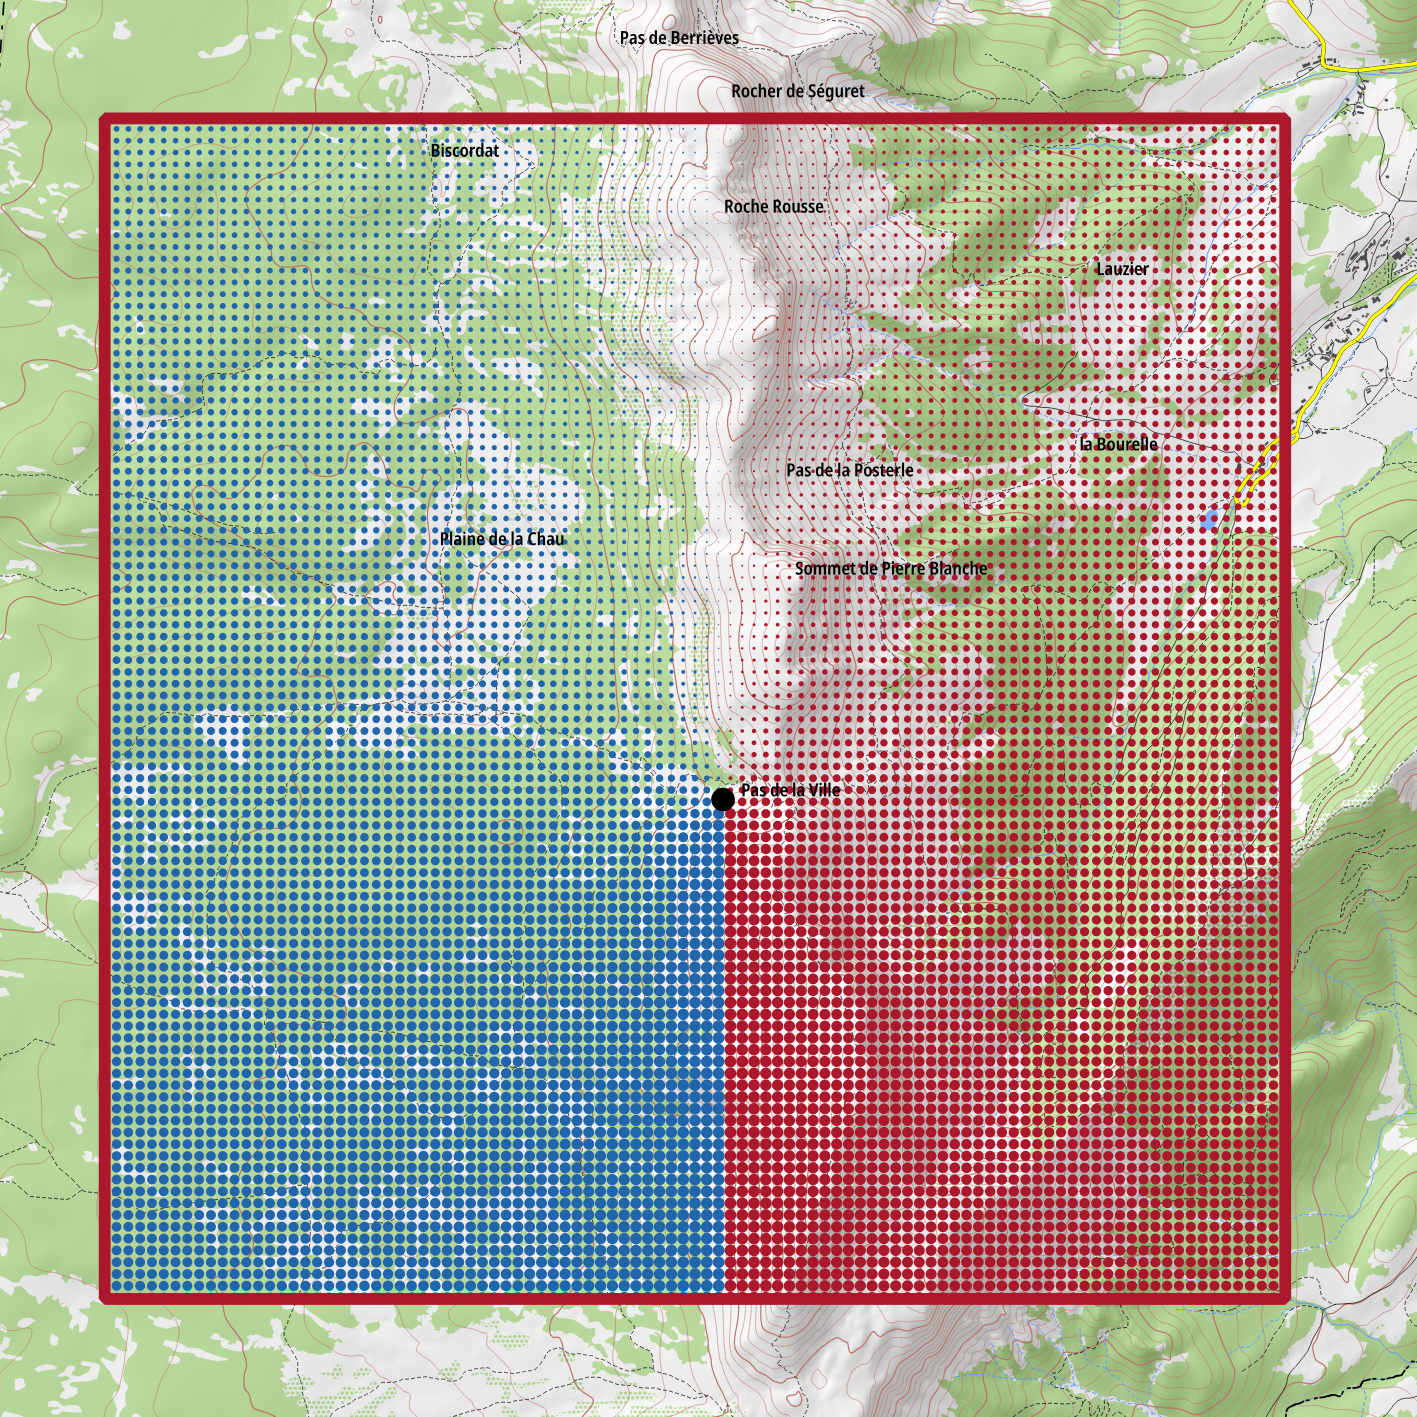
\includegraphics{./figures/EcartNord_PasVille.png}};
  % 
  \begin{scope}
    \node (P2) at ([yshift=-.5cm]image.south east) {};
    \node (P1) at ([yshift=-.5cm]image.south west) {};
    % 
    \node (rect) [anchor=north west, minimum width=1cm,minimum
    height=.25cm] at ([yshift=-.25cm]P1) {}; \path[draw=RdBu-9-1, line
    width=1mm](rect.west) --([xshift=-1ex]rect.south) -- ([xshift=1ex]rect.north)
    -- (rect.east);
    % 
    \node[anchor=west, font=\tiny\vphantom{Ag}, text width = 4cm] at
    ([xshift=1ex]rect.east) {Limite de la \ac{zir}};
    %
    \node[anchor=west, font=\footnotesize\vphantom{Ag}, text width=8cm] at
    (P1 |- 0cm,-1.85cm) {Écart angulaire à la demi-droite passant par
      le \emph{Pas de la Ville} et orientée au nord :};
    %
    \begin{scope}
      \foreach \x [evaluate=\xshift using 1+\x/10, evaluate=\rad using (\x * -.0008) + .05] in {0,...,50}
      {
        \draw[fill=RdBu-9-1,draw=none, below] ([xshift=\xshift cm, yshift=-2.5cm]P1) circle [radius=\rad cm];
      }
      \foreach \x [evaluate=\xshift using 6+\x/10, evaluate=\rad using (\x * .0008) + .01] in {0,...,50}
      {
        \draw[fill=RdBu-9-9,draw=none, below] ([xshift=\xshift cm, yshift=-2.5cm]P1) circle [radius=\rad cm];
      }
      % 
      \path(1,-3) --++ (10,0)
      node[et,pos=0] {\SI{180}{\degre}}
      node[et,pos=.5] {\SI{0}{\degre}}
      node[et,pos=1] {\SI{-180}{\degre}};
    \end{scope}

    % Échelle
    \draw[-] (P2 |- -1cm,-1cm) --++ (-1,0) node[et,pos=.5] {\SI{500}{\meter}};
    % Légende détaillée
    \path (P1) -- (P2) node[pos=.5, yshift=-3cm] {\tiny Pour la légende détaillée du fond topographique voir \autoref{anx:topo_leg}. Sources: BD TOPO 2018, BD ALTI 2018.}; 
  \end{scope}
\end{tikzpicture}
  \caption{Métrique \protect\onto[orla]{Ecart\-Angulaire}, calculée
    pour la spatialisation de la relation de localisation
    \protect\onto[orl]{AuNordDe}. La résolution du raster a
    été réduite de 5 à 50 mètres pour la représentation.}
  \label{fig:veyont_EcartNord}
\end{figure}


% \begin{figure}
%   \centering
%   \begin{tikzpicture}[scale=.7]
  \def\decalageX{-.2}
  \def\decalageY{-.2}
  % Courbe
  \begin{scope}[transparency group]
    % fond
    \begin{scope}
      \path[ffa]  (3,0) -- (4.5, 2) -- (6,0) -- cycle;
    \end{scope}
    % bords
    \begin{scope}
      \path[ffc] (1,.8) -- (3.6,.8) -- (4.5, 2) -- (5.4,.8) -- (8,.8) ;
      \path[ffc_fade_m] (0,.8) -- (1,.8) ;
      \path[ffc_fade] (8,.8) -- (9,.8) ;
    \end{scope}
  \end{scope}
  % Axes X, Y
  \begin{scope}
    % Axe X
    \begin{scope}
      % Axe
      \draw[<->] (0, \decalageX) --++ (9, 0) coordinate (x axis);
      % Graduations
      \foreach \n/\t in {0.5/{},1.5/{},2.5/{400},3.5/{},4.5/{800},5.5/{},6.5/{1200},7.5/{},8.5/{}}
      {
        \draw[-] (\n, \decalageX - .05) --++ (0, .1);
        \node[below, font=\footnotesize] at (\n, \decalageX - .05) {\t};
      }
      % label
      \node[below left, yshift=-.1cm, font=\small] at (x axis)
      {\itshape Distance \normalfont (m)};
    \end{scope}
    % Axe Y
    \begin{scope}
      % Axe
      \draw[-] (\decalageY ,0) --++ (0, 2) coordinate (y axis);
      % Graduations
      \foreach \n/\t in {0/{0},2/{1}}
      {
        \draw[-] (\decalageY -.05, \n) --++ (.1, 0);
        \node[left, font=\footnotesize] at (\decalageY -.05, \n) {\t};
      }
      % Label
      \node[above] at (y axis) {$\mu$};
    \end{scope}
  \end{scope}
  \begin{scope}
    % Seuil 1
    \draw[ffc,line width=.5] (3,\decalageY) -- (3,0);
    \draw[fill, RdBu-9-1] (3,\decalageY) circle (2pt);
    \draw[fill, RdBu-9-1] (3,0) circle (2pt);
    % Seuil 2
    \draw[ffc,line width=.5] (4.5,\decalageY) -- (4.5,2);
    \draw[fill, RdBu-9-1] (4.5,\decalageY) circle (2pt);
    \draw[fill, RdBu-9-1] (4.5,2) circle (2pt);
    % Seuil 3
    \draw[ffc,line width=.5] (6,\decalageY) -- (6,0);
    \draw[fill, RdBu-9-1] (6,\decalageY) circle (2pt);
    \draw[fill, RdBu-9-1] (6,0) circle (2pt);
  \end{scope}
\end{tikzpicture}

%   \caption{XXXX \enquote{Grand Veymont}}
%   \label{fig:fuzzy_veyont_distance}
% \end{figure}



\subsubsection{Au-delà du Pas de la Ville}

La spatialisation de l'indice de localisation \enquote{je suis au-delà
  du Pas de la Ville}, pose certaines difficultés.

La relation de localisation de cet indice est représentée par le
concept \onto[orl]{Après\-Jalon\-Sut\-Itineraire}
(\autoref{anx:orl_dic})

\subsubsection{À 800 mètres du Pas de la Ville}

Ce dernier indice de localisation ne présente pas de difficultés
spécifiques pour être mis en place.


Cette relation est spatialisée à l'aide du \emph{rasteriser}
\onto[orla]{Geometrie}, de la \emph{métrique} \onto[orla]{Distance} et
du \emph{fuzzyficateur} \onto[orla]{Eq\-Val}.

Dans le cas présent, \emph{l'objet de référence} mentionné est le
\emph{Pas de la Ville,} représenté par un ponctuel dans la composante
oronymie de la BDTOPO.


La rasterisation de ce



La \autoref{fig:veyont_distance} représente le résultat du calcul de
la métrique \onto[orla]{Distance} ---~calculée à partir du ponctuel
(rasterisé) représentant le \emph{Pas de la Ville}~--- pour l'ensemble
des positions de la \ac{zir}. Si cette métrique ne présente pas de
caractéristiques particulièrement surprenantes, on peut quand même
noter l'approximation qui est ici faite. Le \emph{Pas de la Ville} est
en effet résumé par un point, alors que le toponyme désigne un
passage, une zone de transition, qui serait sans doute mieux
représentée par un polygone, voire une polyligne. De plus, le point
utilisé n'est pas placé au niveau du point central du Pas de la Ville,
mais à plusieurs centaines de mètres de ce dernier.


\begin{figure}
  \centering
  \begin{tikzpicture}
  \tikzset{et/.style={above,font=\footnotesize\vphantom{Ag}}}
  % 
  \node[inner sep=0pt, anchor=south west] (image) at (0,0){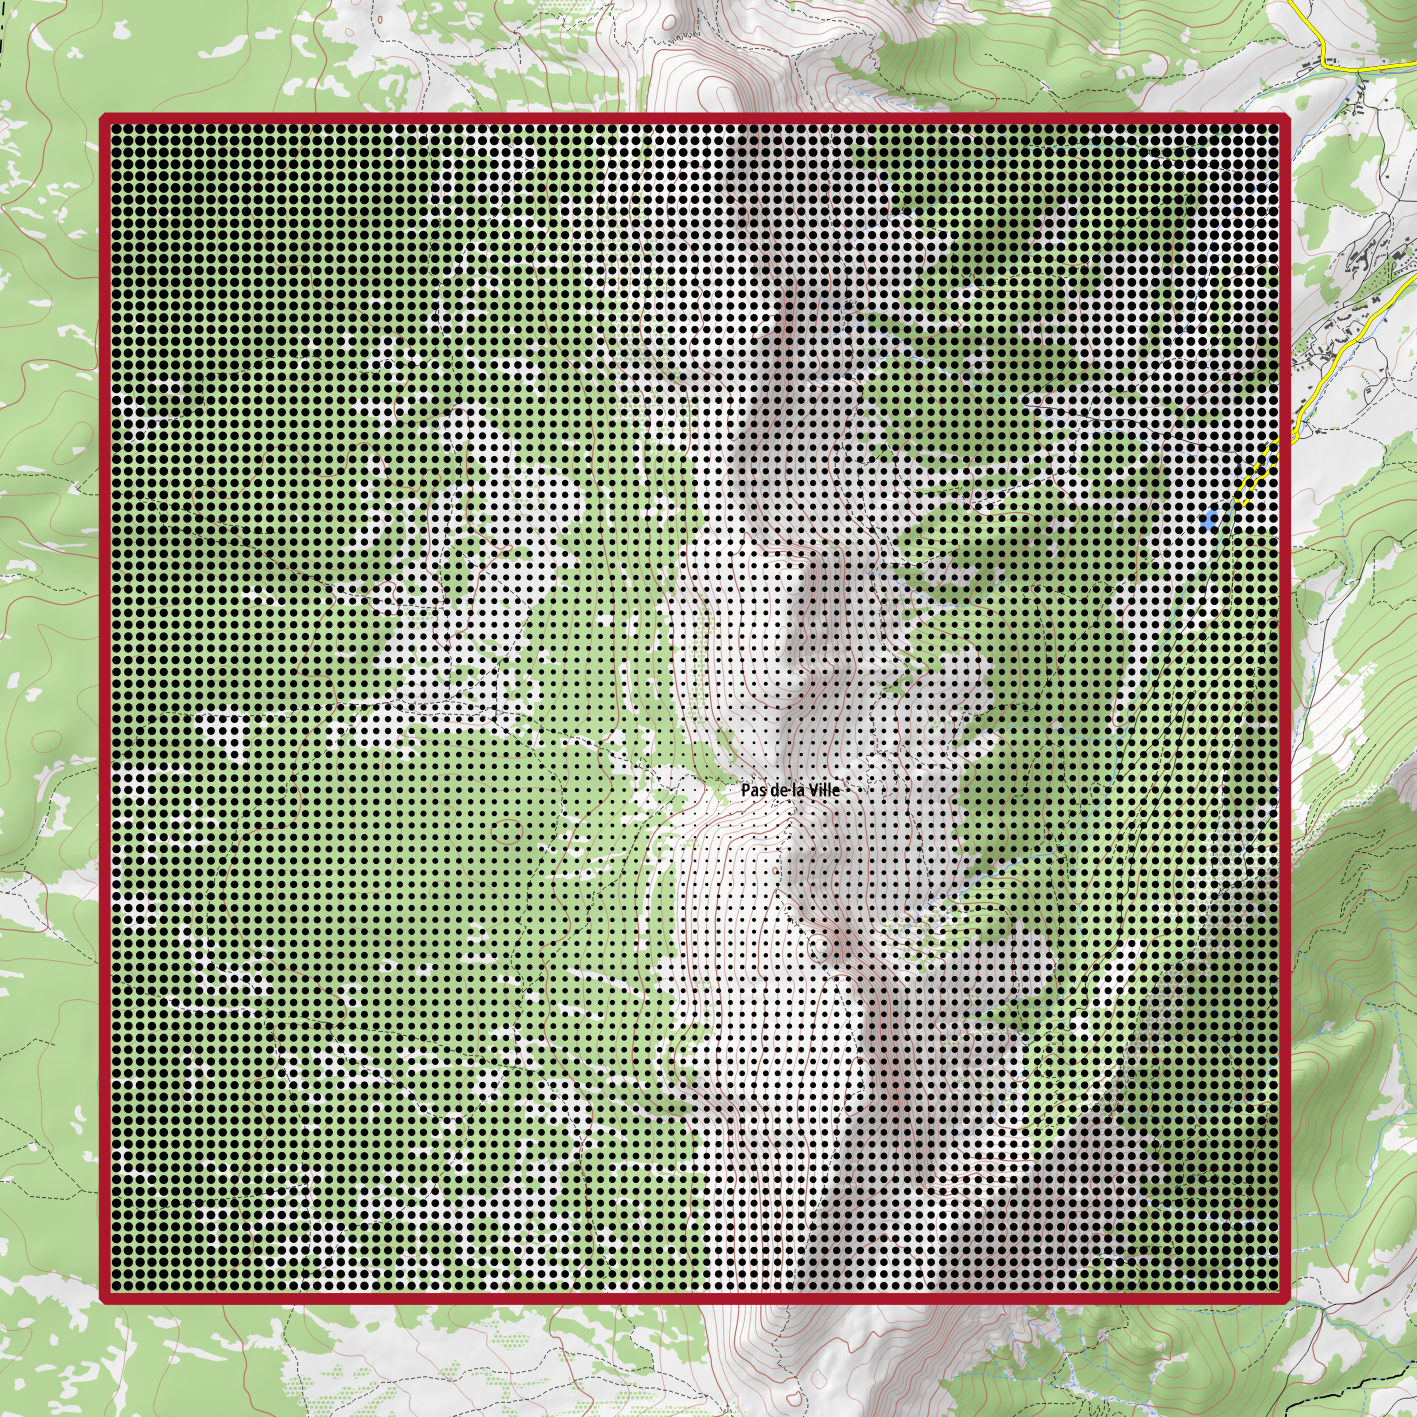
\includegraphics{./figures/Distance_PasVille.png}};
  % 
  \begin{scope}
    \node (P2) at ([yshift=-.5cm]image.south east) {};
    \node (P1) at ([yshift=-.5cm]image.south west) {};
    % 
    \node (rect) [anchor=north west, minimum width=1cm,minimum
    height=.25cm] at ([yshift=-.25cm]P1) {}; \path[draw=RdBu-9-1, line
    width=1mm](rect.west) --([xshift=-1ex]rect.south) -- ([xshift=1ex]rect.north)
    -- (rect.east);
    % 
    \node[anchor=west, font=\tiny\vphantom{Ag}, text width = 4cm] at
    ([xshift=1ex]rect.east) {Limite de la \ac{zir}};
    %
    \node[anchor=west, font=\footnotesize\vphantom{Ag}] at
    (P1 |- 0cm,-1.7cm) {Distance au \emph{Pas de la Ville :}};
    %
    \begin{scope}
      \foreach \x [evaluate=\xshift using 1+\x/10, evaluate=\rad using (\x * .0004) + .01] in {0,...,100}
      {
        \draw[fill=black,draw=none, below] ([xshift=\xshift cm, yshift=-2cm]P1) circle [radius=\rad cm];
      }
      % 
      \path(1,-2.5) --++ (10,0)
      node[et,pos=0] {\SI{0}{\meter}}
      node[et,pos=.5] {\SI{2500}{\meter}}
      node[et,pos=1] {\SI{5000}{\meter}};
    \end{scope}

    % Échelle
    \draw[-] (P2 |- -1cm,-1cm) --++ (-1,0) node[et,pos=.5] {\SI{500}{\meter}};
    % Légende détaillée
    \path (P1) -- (P2) node[pos=.5, yshift=-2.5cm] {\tiny Pour la légende détaillée du fond topographique voir \autoref{anx:topo_leg}. Sources: BD TOPO 2018, BD ALTI 2018.}; 
  \end{scope}
\end{tikzpicture}
  \caption{Métrique \protect\onto[orla]{Distance}, calculée pour la
    spatialisation de la relation de localisation atomique
    \protect\onto[orla]{Distance\-Pla\-ni\-mé\-trique}. La résolution
    du raster a été réduite de 5 à 50 mètres pour la représentation.}
  \label{fig:veyont_distance}
\end{figure}

Pour construire la \ac{zlc} spatialisant cet indice de localisation il
est ensuite nécessaire de \emph{fuzzyfier} la métrique
(\autoref{fig:veyont_distance}) à l'aide du fuzzyficateur
\onto[orla]{Eq\-Val}.

\begin{figure}
  \centering
  \begin{tikzpicture}[scale=.7]
  \def\decalageX{-.2}
  \def\decalageY{-.2}
  % Courbe
  \begin{scope}[transparency group]
    % fond
    \begin{scope}
      \path[ffa]  (3,0) -- (4.5, 2) -- (6,0) -- cycle;
    \end{scope}
    % bords
    \begin{scope}
      \path[ffc] (1,.8) -- (3.6,.8) -- (4.5, 2) -- (5.4,.8) -- (8,.8) ;
      \path[ffc_fade_m] (0,.8) -- (1,.8) ;
      \path[ffc_fade] (8,.8) -- (9,.8) ;
    \end{scope}
  \end{scope}
  % Axes X, Y
  \begin{scope}
    % Axe X
    \begin{scope}
      % Axe
      \draw[<->] (0, \decalageX) --++ (9, 0) coordinate (x axis);
      % Graduations
      \foreach \n/\t in {0.5/{},1.5/{},2.5/{400},3.5/{},4.5/{800},5.5/{},6.5/{1200},7.5/{},8.5/{}}
      {
        \draw[-] (\n, \decalageX - .05) --++ (0, .1);
        \node[below, font=\footnotesize] at (\n, \decalageX - .05) {\t};
      }
      % label
      \node[below left, yshift=-.1cm, font=\small] at (x axis)
      {\itshape Distance \normalfont (m)};
    \end{scope}
    % Axe Y
    \begin{scope}
      % Axe
      \draw[-] (\decalageY ,0) --++ (0, 2) coordinate (y axis);
      % Graduations
      \foreach \n/\t in {0/{0},2/{1}}
      {
        \draw[-] (\decalageY -.05, \n) --++ (.1, 0);
        \node[left, font=\footnotesize] at (\decalageY -.05, \n) {\t};
      }
      % Label
      \node[above] at (y axis) {$\mu$};
    \end{scope}
  \end{scope}
  \begin{scope}
    % Seuil 1
    \draw[ffc,line width=.5] (3,\decalageY) -- (3,0);
    \draw[fill, RdBu-9-1] (3,\decalageY) circle (2pt);
    \draw[fill, RdBu-9-1] (3,0) circle (2pt);
    % Seuil 2
    \draw[ffc,line width=.5] (4.5,\decalageY) -- (4.5,2);
    \draw[fill, RdBu-9-1] (4.5,\decalageY) circle (2pt);
    \draw[fill, RdBu-9-1] (4.5,2) circle (2pt);
    % Seuil 3
    \draw[ffc,line width=.5] (6,\decalageY) -- (6,0);
    \draw[fill, RdBu-9-1] (6,\decalageY) circle (2pt);
    \draw[fill, RdBu-9-1] (6,0) circle (2pt);
  \end{scope}
\end{tikzpicture}

  \caption{XXXX \enquote{Grand Veymont}}
  \label{fig:fuzzy_veyont_distance}
\end{figure}



\begin{figure}
  \centering
  \input{./figures/Distance_GrandVeymont.tex}
  \caption{XXXX \enquote{Grand Veymont}}
  \label{fig:Distance_GrandVeymont}
\end{figure}




\subsubsection{Fusion des zones de localisation compatibles}

À la suite de la spatialisation des différents indices de localisation
et de la composition des 

\subsection{Critique de la modélisation}
\label{subsec:9-2-3}

\tdi{Impact de la position du toponyme "pas de la ville" sur la
  modélisation}

Un autre problème notable est l'impact que peut avoir la géométrie des
objets de référence sur le résultat de la spatialisation. Par exemple,
l'indice de localisation : \enquote{À \SI{800}{\meter} du Pas de la
  Ville} a été spatialisé en calculant la métrique
\onto[orla]{Distance} à partir du ponctuel plaçant l'oronyme
\enquote{Pas de la Ville} dans la base de données. Or, la
représentation d'un géotype étendu, comme un pas ou une crête, par un
point est une approximation conséquente, impactant fortement la
spatialisation.


%%% Local Variables:
%%% mode: latex
%%% TeX-master: "../../../../main"
%%% End:
